\chapter{About the Template}
%\label{chapter:title}

This template aims to simplify and improve the (Xe)LaTeX report/thesis template by OST with the following three main design principles:

\begin{itemize}
  \item \textbf{Simplicity First:} A class file that has been reduced by nearly 70\% to simplify customization;
  \item \textbf{Effortless:} A careful selection of common packages to get started immediately;
  \item \textbf{Complete:} Ready-to-go when it comes to the document and file structure.
\end{itemize}

\noindent This template works with pdfLaTeX, XeLaTeX and LuaLaTeX. In order to adhere to the OST house style, either XeLaTeX or LuaLaTeX is required, as it supports TrueType and OpenType fonts. BibLaTeX is used for the bibliography with as backend biber. Please visit \url{https://norukh.github.io/report/} for the full documentation.

\section*{Documentation (Abridged)}

As a report/thesis is generally a substantial document, the chapters and appendices have been separated into different files and folders for convenience. The folders are based on the three parts in the document: the frontmatter, mainmatter and appendix. All files are inserted in the main file, \texttt{report.tex}, using the \texttt{\textbackslash input\{filename\}} command. The document class, which can be found in \texttt{ost-report.cls}, is based on the book class. 

The template will automatically generate a cover when the \texttt{\textbackslash makecover} command is used. The title, subtitle and author will also be present on the title page. To give greater flexibility over the title page, the layout is specified in \texttt{title-report.tex}. A title page for theses is also available: \texttt{title-thesis.tex}. Change the corresponding \texttt{\textbackslash input\{...\}} command in the main file to switch. 

The bibliography has been set up in \texttt{report.tex} to allow for easy customization. It is included in the table of contents and renamed to 'References' using the \texttt{heading=bibintoc} and \texttt{title=References} options of the \texttt{\textbackslash printbibliography} command respectively. If you would like to use a different .bib file, change the command \texttt{\textbackslash addbibresource{report.bib}} accordingly.

\emph{→ Visit \url{https://norukh.github.io/report/} for the full documentation.}

\begin{figure}[h]
  \centering
  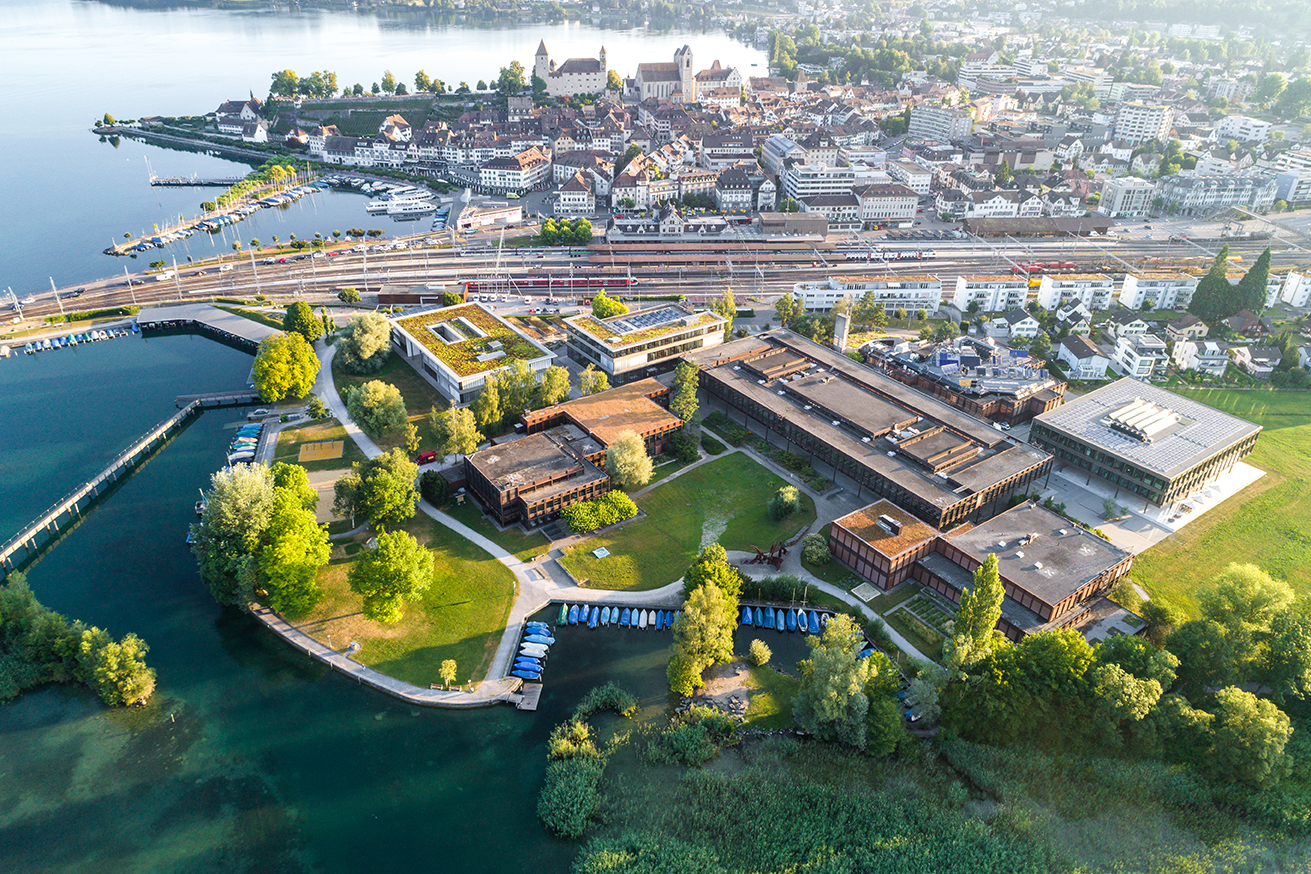
\includegraphics[width=0.95\linewidth]{figures/ost-campus-rj.jpg}
  \caption{OST Campus Rapperswil}
\end{figure}

\section*{License}

The origin of this template is the report/thesis template by Daan Zwaneveld, which is licensed under CC BY-NC 4.0.
This template has been adopted by Nico Fehr to the OST design and is licensed under CC BY-NC 4.0 as well. To view a copy of this license, visit \url{https://creativecommons.org/licenses/by-nc/4.0/}. No attribution is required in PDF outputs created using this template.